\begin{center}
\footnotesize
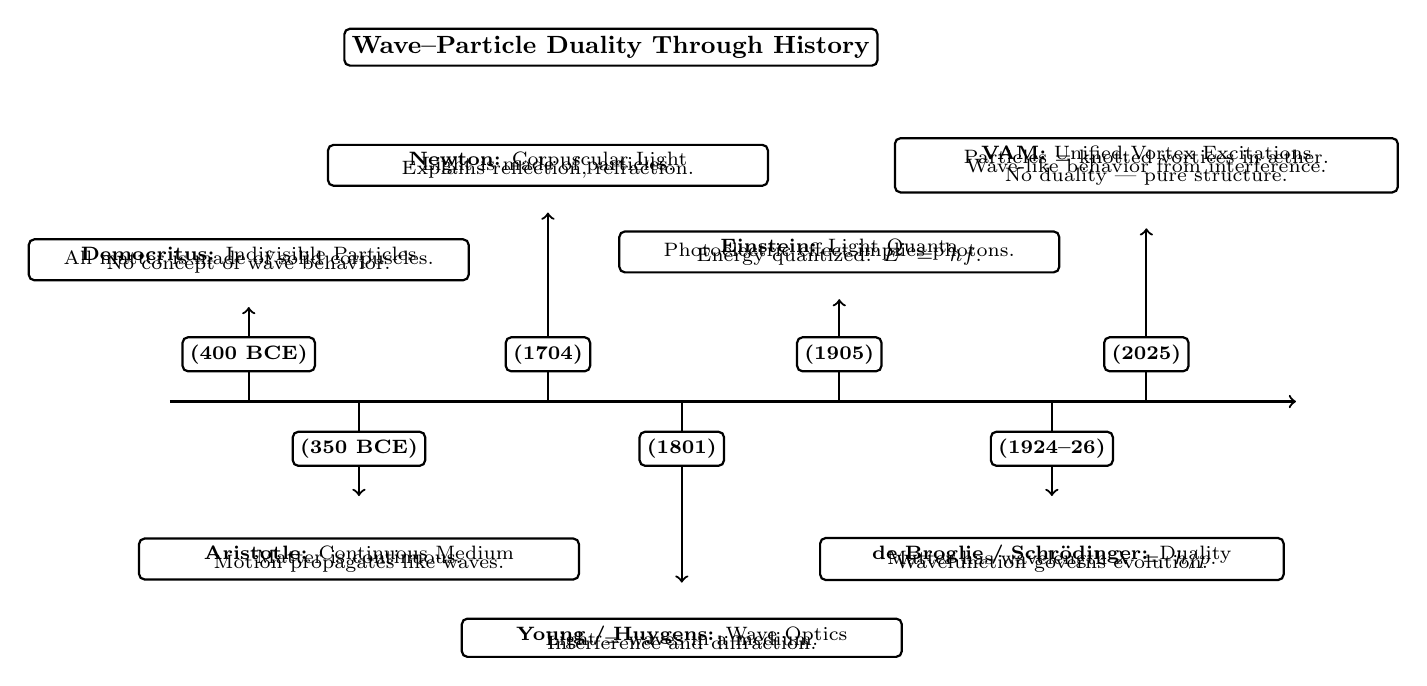
\begin{tikzpicture}
\scriptsize

% Timeline base
\draw[->, thick] (-1,0) -- (13.3,0);

% Arrows above timeline
\draw[->, thick] (0,0) -- (0,1.2);       % Democritus
\draw[->, thick] (3.8,0) -- (3.8,2.4);   % Newton
\draw[->, thick] (7.5,0) -- (7.5,1.3);   % Einstein
\draw[->, thick] (11.4,0) -- (11.4,2.2); % VAM

% Arrows below timeline
\draw[->, thick] (1.4,0) -- (1.4,-1.2);     % Aristotle
\draw[->, thick] (5.5,0) -- (5.5,-2.3);     % Young/Huygens
\draw[->, thick] (10.2,0) -- (10.2,-1.2);   % de Broglie

% --- Date labels ---
\node[draw, thick, rounded corners=2pt, fill=white, align=center, font=\bfseries ] at (0, .6)   {(400 BCE)};
\node[draw, thick, rounded corners=2pt, fill=white, align=center, font=\bfseries ] at (3.8, .6) {(1704)};
\node[draw, thick, rounded corners=2pt, fill=white, align=center, font=\bfseries ] at (7.5, .6) {(1905)};
\node[draw, thick, rounded corners=2pt, fill=white, align=center, font=\bfseries ] at (11.4, .6){(2025)};

\node[draw, thick, rounded corners=2pt, fill=white, align=center, font=\bfseries ] at (1.4,- .6) {(350 BCE)};
\node[draw, thick, rounded corners=2pt, fill=white, align=center, font=\bfseries ] at (5.5,- .6) {(1801)};
\node[draw, thick, rounded corners=2pt, fill=white, align=center, font=\bfseries ] at (10.2,- .6) {(1924--26)};

% Timeline label
\node[draw, thick, fill=white, rounded corners=2pt, font=\small] at (4.6,4.5) {\textbf{Wave–Particle Duality Through History}};

% --- Democritus ---
\node[draw, rounded corners=2pt, thick, align=center, fill=white, text width=5.4cm] at (0,1.8) {
\textbf{Democritus:} Indivisible Particles \\[-0.8em]
All matter is made of solid corpuscles. \\[-0.8em]
No concept of wave behavior.
};

% --- Newton ---
\node[draw, rounded corners=2pt, thick, align=center, fill=white, text width=5.4cm] at (3.8,3.0) {
\textbf{Newton:} Corpuscular Light \\[-0.8em]
Light is made of particles. \\[-0.8em]
Explains reflection, refraction.
};

% --- Einstein ---
\node[draw, rounded corners=2pt, thick, align=center, fill=white, text width=5.4cm] at (7.5,1.9) {
\textbf{Einstein:} Light Quanta \\[-0.8em]
Photoelectric effect implies photons. \\[-0.8em]
Energy quantized: \( E = hf \).
};

% --- VAM ---
\node[draw, rounded corners=2pt, thick, align=center, fill=white, text width=6.2cm] at (11.4,3.0) {
\textbf{VAM:} Unified Vortex Excitations \\[-0.8em]
Particles = knotted vortices in æther. \\[-0.6em]
Wave-like behavior from interference. \\[-0.6em]
No duality — pure structure.
};

% --- Aristotle ---
\node[draw, rounded corners=2pt, thick, align=center, fill=white, text width=5.4cm] at (1.4,-2.0) {
\textbf{Aristotle:} Continuous Medium \\[-0.8em]
Matter is continuous. \\[-0.8em]
Motion propagates like waves.
};

% --- Young / Huygens ---
\node[draw, rounded corners=2pt, thick, align=center, fill=white, text width=5.4cm] at (5.5,-3.0) {
\textbf{Young / Huygens:} Wave Optics \\[-0.8em]
Light = waves in a medium. \\[-0.8em]
Interference and diffraction.
};

% --- de Broglie / Schrödinger ---
\node[draw, rounded corners=2pt, thick, align=center, fill=white, text width=5.7cm] at (10.2,-2.0) {
\textbf{de Broglie / Schrödinger:} Duality \\[-0.8em]
Matter has wavelength \( \lambda = h/p \). \\[-0.8em]
Wavefunction governs evolution.
};

\end{tikzpicture}
\captionof{figure}{Development of wave–particle duality: from atomistic corpuscles and wave optics, through quantum superposition, to VAM’s unified vortex excitation model.}
\end{center}